\subsection{Caso de uso 3: Consultar perfil} \label{cu3}
\subsubsection{Resumen}

\subsubsection{Descripción}
\begingroup
\setlength{\LTleft}{-10cm plus -1fill}
\setlength{\LTright}{\LTleft}
\begin{center}
  \captionof{table}{Caso de uso 3: Consultar perfil} \label{tab:cu3}
  \begin{longtable}{| p{3.5cm} | p{11.5cm} |}
        \hline
        \textbf{Versión} &  0.1\\
        \hline 
        \textbf{Autor} & \\
        \hline
          \textbf{Estatus} & Edición \\
        \hline  
          \textbf{Fecha de último estatus} & 31 de marzo de 2017 \\
        \hline
      \multicolumn{2}{c |}{\large{Atributos:}} \\
        \hline
          \textbf{Actor}  &  Usuario y Sub-Usuario\\
        \hline  
          \textbf{Propósito} &  Permite a los actores consultar su perfil \\
        \hline
          \textbf{Disparador} & Al presionar el botón BTN en la vista IU Inicio\\
        \hline  
          \textbf{Entradas} & \\
        \hline  
          \textbf{Salidas} &  
		\begin{itemize}
	              \item Interna: Se mostrará la IU Perfil
	        \end{itemize} \\
        \hline  
          \textbf{Precondiciones} & 
		\begin{itemize}
	              \item I\textbf{nterna:} El actor debe estar registrado en el sistema
	            \end{itemize} \\
        \hline  
          \textbf{Postcondiciones} &
		\begin{itemize}
	              \item Interna: Se mostrará la IU Perfil con el cual podrá consultar sus datos
	            \end{itemize} \\
        \hline
          \textbf{Reglas de negocio} & 
		\begin{itemize}
	         	  \item {\hyperref[rnr_01]{RNE 01: Cuenta válida}}
		 \end{itemize} \\
        \hline
          \textbf{Mensajes} & \\
        \hline
          \textbf{Tipo} & Secundario\\
        \hline      
  \end{longtable}
\end{center}
\endgroup

\subsubsection{Trayectorias del caso de uso}
\textbf{Trayectoria principal}
\begin{enumerate}
 \item {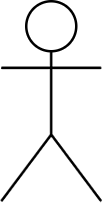
\includegraphics[scale=.1]{Capitulo3/img/actor.png} Ingresa el actor a la aplicación móvil.}
\item {
\includegraphics[scale=.05]{Capitulo3/img/proceso.png} Se muestra la vista IU Inicio.}
\item {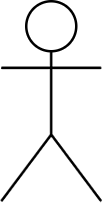
\includegraphics[scale=.1]{Capitulo3/img/actor.png} Presiona el botón de Iniciar sesión.}
\item {
\includegraphics[scale=.05]{Capitulo3/img/proceso.png} Se muestra la vista IU Inicio.}
\item {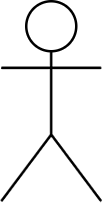
\includegraphics[scale=.1]{Capitulo3/img/actor.png} Selecciona el usuario la opción de \textit{Consultar perfil}}
\item {
\includegraphics[scale=.05]{Capitulo3/img/proceso.png} Se muestra la IU Perfil}
  \textit{Fin de caso de uso} \\  
\end{enumerate}

\textbf{Trayectoria alternativa} \phantomsection\label{cu_ta_} \\
\textbf{Condición:} \\
 \begin{enumerate}[label=\arabic*]
    \item {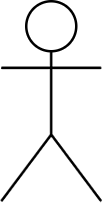
\includegraphics[scale=.1]{Capitulo3/img/actor.png} }
    \item {
\includegraphics[scale=.05]{Capitulo3/img/proceso.png}}
    \item {Continua en el paso 4 de la trayectoria principal.} \\
    \textit{Fin de trayectoria} \\
\end{enumerate}

\subsubsection{Puntos de extensión}
\noindent \textbf{Causa de la extensión: El actor, de tipo Usuario o Sub-Usuario, seleccionó \textit{Editar perfil}} \\
\textbf{Región de la trayectoria:} \hyperref[cu3_ta_]{Trayectoria alternativa } \\
\textbf{Extiende a:} \hyperref[cu3]{CU 3 Consultar perfil}

\noindent \textbf{Causa de la extensión:} El actor, de tipo de Usuario o Sub-Usuario, selecciono \textit{Editar perfil} \\
\textbf{Región de la trayectoria:} \hyperref[cu3_3_ta_e]{Trayectoria alternativa e} \\
\textbf{Extiende a:} \hyperref[cu3]{CU 3 Consultar Perfil}
